\documentclass{statsoc}
\usepackage[english]{babel}
\usepackage[a4paper]{geometry}
\usepackage{bm}
\usepackage{amsmath}
\usepackage{amssymb}
%%\usepackage{graphics}
\usepackage[authoryear]{natbib}
\usepackage{relsize}
%\usepackage{color}
\usepackage[table]{xcolor}
\usepackage{multirow}
\usepackage{mathptmx}
%\usepackage{transparent}
%\usepackage{xcolor}
%\usepackage{efbox}
\usepackage{float}
%\usepackage{subfig}
%
%\usepackage{hvfloat}
%\usepackage{booktabs}
%\usepackage[font=footnotesize]{caption}
\usepackage{etoolbox}
\usepackage{url}
\usepackage[table]{xcolor}
\usepackage{array}
\usepackage{tikz}
\usetikzlibrary{trees}
\DeclareGraphicsExtensions{.pdf,.png,.jpg,.eps} 


\makeatletter
\patchcmd{\@makecaption}
{\parbox}
{\advance\@tempdima-\fontdimen2\font\parbox} % decrease the width!
{}{}
\makeatother  

\usepackage{graphicx}
\usepackage[caption=false]{subfig}
\usepackage{enumerate}
\usepackage{comment}
\usepackage{float}

\newcommand\Pair[4]{%
  \arrayrulecolor{cyan!60!black!40}%
  \arrayrulewidth=1pt
  \renewcommand\extrarowheight{1.5pt}%
  \begin{tabular}{|p{2cm}|>{\centering\arraybackslash}p{10pt}|}
  \hline
  \rowcolor{cyan!60!black!10}\textcolor{red!60!black}{#1} & \textcolor{red!60!black}{#2} \\
  \hline 
  \rowcolor{cyan!60!black!10}\textcolor{red!60!black}{#3} & \textcolor{red!60!black}{#4} \\
  \hline
  \end{tabular}%
}


\usepackage[colorinlistoftodos,textwidth=2.2cm, textsize=tiny]{todonotes}
\setlength{\marginparwidth}{2.5cm}
\newcommand{\leo}[1]{\todo[linecolor=orange, size=\footnotesize, backgroundcolor=orange!25,bordercolor=orange]{Leo: #1}}
\newcommand{\jonah}[1]{\todo[linecolor=blue, size=\footnotesize, backgroundcolor=blue!25,bordercolor=orange]{Jonah: #1}}



\newtheorem{thm}{Theorem}

\title[]{Prediction is not everything, but everything is prediction}
\author[Egidi and Gabry]{Leonardo Egidi}
\address{Dipartimento di Scienze Economiche, Aziendali, Matematiche e Statistiche `Bruno de Finetti',
	Universit\`{a} degli Studi di Trieste,
	Trieste,
	Italy.}
\email{legidi@units.it}
\author[Egidi and Gabry]{Jonah Sol Gabry}
\address{Department of Statistics, Columbia University, New York,
USA.}
\email{jgabry@gmail.com}
 
 


\begin{document}

\maketitle

\begin{abstract}
Prediction is an unavoidable task for data scientists, and over the last few decades, statistics and machine learning have become the most popular `prediction weapons' in many fields. However, prediction should always be associated with a measure of uncertainty - because from it  we can only reconstruct and 
falsify the model/algorithm decisions. Machine learning methods offer many point predictions,  but they rarely yield a measure of uncertainty, whereas statistical 
models usually do a poor job of communicating predictive results.
According to Popper’s falsification philosophy, natural and physical sciences can be falsified on the grounds of incorrect predictions: however  this is not always true in the social sciences.
We move then to a weak instrumentalist philosophy: Predictive accuracy is not always constitutive of scientific success, especially in the social sciences.\\

\emph{Keywords}: Prediction; Popper’s falsification philosophy; Weak instrumentalism; Predictive accuracy; Machine learning

\end{abstract}

\section{Introduction}

As motivated by falsificationism
\citep{popper1934logic} and many philosophers of science, prediction has a primary role in the progress of science; however, this is often controversial---see \cite{kuhn1962structure} and \cite{lakatos1976falsification} for some criticisms. Popper argues 
that theories, to be scientific, must be falsifiable on the ground of their  predictions: wrong predictions should perhaps push scientists to reject their theories or to 
re-formulate them, conversely exact predictions should corroborate a scientific theory. Popper's philosophy is instrumentalist 
in a strong sense \citep{hitchcock2004prediction} when applied to physical and natural sciences: predictive accuracy is constitutive of scientific success, not only symptomatic of it, and  prediction works as a confirmation theory tool for science.   
% it is worth noting that Popper's point of 
%view is oriented towards physics and natural sciences, whereas he is more and more skeptical about prediction in social sciences \citep{popper1944poverty, popper1945poverty}.

Since the 1940s, with the growing availability of fast computers and the use of simulation routines, science expanded its boundaries and extended the existing frameworks in new dimensions; for instance, think of the Manhattan project in Los Alamos, when the problem of neutron diffusion in fissionable material allowed Stanislaw Ulam and Nicholas Metropolis to invent and develop Markov Chain Monte Carlo Methods through the ENIAC computer. In particular, the birth 
and growth of probabilistic and statistical methods have made the `debut of science in society' possible, whereas the growing ability of data and the development of sophisticated computational 
tools starting from the 1950s and 1960s opened the door to data science revolution; the 1990s transformed  data science into a 
global oracle, and data scientists gained more credibility as the availability of  modern machinery grew.

For many of us, data science and statistical methods 
are scientific with tools designed to formulate a theory (model) from some evidence (data) and generalize this hypothesis by induction.
Over the last few decades, statistics and machine learning (ML) have become the most popular `prediction weapons' for both social and natural sciences, including frameworks such as weather's forecasting, presidential elections, planets' motions, global warming, gross domestic product, etc. However, there is often a clear separation between these two fields: statistics is usually seen as a discipline that extracts information from  current data, whereas ML is usually designed to predict new events.  However, many times the right weapons are embraced by the wrong people. The predictive power in statistics is a small elegant 
gun, with small bullets and good properties, whereas in ML it is a bazooka, with  big bullets and devastating effectiveness. The statistician knows the gun's details and how it is used, the machine learner is rarely aware of the bazooka's properties. Most literature on ML methods \citep{breiman2001statistical} is based on their ability to successfully predict test set 
data, but (almost) nothing is said about the technical assumptions required to tune/build the algorithms; conversely, many statistical methods are claimed to be good upon the check of 
their residuals on the training data, but rarely on the ground of some forecasting abilities on holdout samples.
 
%As already mentioned, there is much debate about the role of 
%prediction in the scientific process;  many scientists and philosophers of science, with the pioneering work of Popper,  consider prediction as a confirmation theory approach for 
%science. 
%In this paper, we revise this position by considering first the role of prediction in the progress of science from Galileo Galilei to Albert Einstein; then, we analyse the role of prediction in modern statistical learning methods, by drawing an analogy between the steps required to formulate a scientific theory and those required to set up a Bayesian model.

The main novelty of this paper is the \emph{weak instrumentalist} position for prediction, under which predictive accuracy is constitutive of scientific success only when the 
underlying statistical methods are falsifiable and transparently designed to predict out-of-sample events.  In other words, there are many contexts, especially in the social sciences, where falsification through the prediction's fallacy should be replaced by a more consistent idea of falsification: we believe this position may be beneficial for the so-called hard sciences as well.  On one hand, mathematical and quantitative laws formulated by Galilei and Newton 
were physical and deterministic with which  particular future facts could have been predicted with absolute precision; On the other hand, probabilistic and statistical laws designed 
to describe human behavior and social facts are stochastic laws, with which particular future  events could be predicted with an intrinsic amount of uncertainty. 
Of course, as statisticians we want to do our best in predict future social events, but we cannot entirely evaluate a model's performance only on the ground of its predictive accuracy. Using Popper's terminology, incorrect social sciences predictions should not be the only tool to falsify a theory.

Prediction is an unavoidable task for scientists working 
with data, but it is not all we need, especially when framed in social science frameworks; moreover, prediction should always be associated with a measure of variability, because from variability only we are able to reconstruct and 
falsify the model/algorithm decisions. ML methods offer many point-predictions,  but they rarely yield a measure of uncertainty, whereas statistical 
models, when predicting new items, usually do a bad job in communicate results poorly. Weak instrumentalist philosophy should push statisticians to embrace the bazooka more when needed, and the machine learners to use a more precise gun when a bazooka is unnecessary.

In Section~\ref{sec:pred} we revise the steps required to formulate a scientific theory and review the role of prediction for natural sciences from Galilei's law of falling bodies to 
Albert Einstein's general relativity. We also analyze the confirmation theory approach, both in natural and social sciences. In Section~\ref{sec:role}, we focus on 
predictions for statistical learning, while a weak instrumentalist philosophy is detailed in Section~\ref{sec:instr}. Section~\ref{sec:world} proposes an applied example for the football Russia World Cup 2018, and Section~\ref{sec:concl} concludes.


\section{Prediction for science or science for prediction?}
\label{sec:pred}

\subsection{Is prediction part of science design?}

\color{black}

The main stages required to formulate a scientific law are summarized by \cite{russell2017scientific} as follows:
(1) observation of some relevant facts,
(2) formulation of a hypothesis underlying and explaining the previously mentioned facts, and
(3) deduction of some consequences from this hypothesis.
As suggested by \cite{russell2017scientific}, the modern scientific method was born with Galileo Galilei, father of the law of falling bodies, and with Johannes Kepler, who discovered the three laws of planetary motion:
%
 \begin{quote}
 \emph{
Scientific method, as we understand it, comes into the
world full-fledged with Galileo (1564-1642), and, to a
somewhat lesser degree, in his contemporary, Kepler
(1571-1630). [...] They proceeded from observation of
particular facts to the establishment of exact quantitative
laws, by means of which future particular facts could be
predicted.
}
\end{quote}
%
 Then, the law of universal gravitation of Isaac Newton embodied the two previous theories, whereas the theory of the general relativity of Albert Einstein generalized  Newton's theory.
Thus, in the last 500 years, physics---and, more generally, science---advanced by falsification and generalization of previous theories, by providing new and more exciting theories to predict new natural facts and highlighting the confirmation nature of prediction. In general,  as \cite{hitchcock2004prediction} argue,   mathematical descriptions of the 
invariant behaviour of a physical phenomenon are essentially predictive: further experiments and observations can validate these theories. 

However, prediction's link with scientific laws is  more ambiguous than what people are usually inclined to think. The following questions arise: Is prediction a central step in science? 
Is prediction a relevant aim of science? 
A negative answer to the first question could be seen in disagreement with some 
\emph{instrumentalist} scientists, who would claim that, from an instrumental perspective, predictive success is not merely \emph{symptomatic} of scientific success, is also 
\emph{constitutive} of scientific success \citep{hitchcock2004prediction}. A more sophisticated answer could be  that prediction is not explicitly part of the formulation of a 
scientific hypothesis (1)--(3) \emph{at the time the law is posed}, but it becomes relevant and relevant as science advances; the chain of events that brought Newton to 
generalize the theories of Galilei and Kepler first, and Einstein to revisit the gravitational law of Newton then, was supposedly based on the fallacy of some predictions, and it gained sense 
only \emph{ex-post}. The fact that the bodies in proximity to the earth surface were revealed by Newton to not fall exactly with a constant acceleration---the acceleration slightly 
rises as they get closer to the earth---did not make Galilei's law of constant acceleration for falling bodies less scientific, or totally wrong from a scientific point of view. Scientific falsification detected by wrong predictions \citep{popper1934logic} is a powerful and exceptional tool, but in this paper we caution  its abuse/misuse. 

Scientific predictions has recently become popular not only in the context of physics and natural science, but for the social sciences as well. Steps (1)--(3) above are widely used by social scientists and statisticians to build consistent theories about human and social behaviurs: Recently, the need to build a quantitative population's laws with the aim to mimic physical nature's laws emerged.  However, the role played by 
prediction in social sciences is even more obscure \citep{popper1944poverty, popper1945poverty} and much more controversial than for the natural sciences, though data scientists are increasingly asked to build 
`weapons of mass prediction' in varying social contexts. 
 %The way in which they formulate their theories underlying  some data follows in the majority of the circumstances the scheme 
%outlined by Bertrand Russell and reported at the beginning of this section: the stage of `hypothesis formulation' is vague here, but may be interpreted either in form of the 
%classical statistical testing procedure, or in terms of a model to be checked.
Perhaps, the actual outcome may be far away from the predictions: Trump's win in the US 
presidential elections, Brexit, and the Leicester's Premier League's win were very low-probability events, but they all occurred in 2016. Can all of these rare events falsify the finest algorithms and models designed to not predict their occurrence? Our naive and tentative answer is no, they cannot. We give more details on this in the next section.



%,: (out-of-sample) predictions are a task of science, but only (in-sample) predictions are constitutive of scientific success.

\subsection{Prediction as a confirmation theory approach}

%\textcolor{blue}{Popper, Kuhn, Mayo}

For \cite{popper1934logic}, a theory is scientific only if it is falsifiable, where the falsification of a theory is meant to be the possibility of comparing its predictions 
with the observed data. In his view, theories whose predictions conflict with any observed evidence must be rejected: prediction corroborates (or confirms) a theory when it survives 
an attempt at falsification; prediction delegitimizes a theory when it does not pass the falsification test.

The confirmation nature of prediction is crucial in the natural sciences, such as physics. In general,  as \cite{hitchcock2004prediction} argue,   mathematical descriptions of the 
invariant behavior of a physical phenomenon---such as Newton's and Keplero's laws, or Maxwell's equations---are essentially predictive, further experiments and observations can validate these theories. 

A well-known historical example of predictive confirmation in chemistry dates back to the middle of the 19th century---see \cite{maher1988prediction} for  details. At that time, more than 60 chemical elements were known, and new ones continued to be discovered. Some prominent chemists attempted to determine their atomic weights, 
densities and other properties, by collecting experimental observations. In 1871, the Russian chemist Dmitri Mendeleev noticed that arranging the elements by their atomic 
weights, valences and particular chemical properties tended to show periodical recurrences. He found some gaps in the pattern and argued that these missing values corresponded to 
some existing elements that had not yet been discovered. He named three of these elements (eka-aluminium, eka-boron, and eka-silicon) and gave some detailed descriptions of their 
properties. Despite the skepticism of the scientific community,  French Paul-Emile Lecoq de Boisbaudran in 1874,  Swedish Lars Fredrik Nilson in 1878, and  German Clemens 
Winkler in 1886 discovered three elements that corresponded to descriptions of eka-aluminium, eka-boron, and exa-silicon: these three elements are now respectively 
known as gallium, scandium and germanium.  Mendeleev's predictive ability was remarkable---the Royal Society awarded him the Davy Medal in 1882---, and the newly discovered elements represented pieces of evidence that confirmed the theory.

Predictive confirmation is still ambiguous in the social sciences. As argued by \cite{popper1944poverty, popper1945poverty} and \cite{sarewitz1999prediction}, the social sciences 
have long tried to emulate physical sciences in developing invariant mathematical laws of human behavior and interaction to predict economics quantities, elections, policies, etc.; 
many scholars agreed that a social theory should be judged on its power to predict \citep{friedman1953essays}. 

However, we believe that social science predictions require more motivations to validate underlying theories. In the 2016 United States presidential election   Donald Trump (Republican) defeated   Hillary Clinton (Democrat) by winning the electoral college (304 vs 227), but gaining a lower voter percentage (46.1\% vs 48.2\%). According to various online poll aggregators, Clinton was given a 65\% or 80\% or 90\% chance of winning the electoral college.  As \cite{gelman2016elections} argues:

\begin{quote}
\emph{
 These probabilities were high because Clinton had been leading in the polls for months; the probabilities were not 100\% because it was recognized that the final polls might be off by quite a bit from the actual election outcome. Small differences in how the polls were averaged corresponded to large apparent differences in win probabilities; hence we argued that the forecasts that were appearing, were not so different as they seemed based on those reported odds. The final summary is that the polls were off by about 2\% (or maybe 3\%, depending on which poll averaging you’re using), which, again, is a real error of moderate size that happened to be highly consequential given the distribution of the votes in the states this year.
 }
\end{quote}
%
In November 2016, many modelers including Nate Silver, the founder of the well-known FiveThirtyEight blog (\url{https://fivethirtyeight.com}), failed to predict Trump's win. However, it is naive to conclude that these models failed because their underlying mechanism was wrong; rather, political science predictions cannot  act as theory's only confirmation tools for many reasons, for instance nonresponse and voter turnout, as explained by \cite{gelman2016elections2}:

\begin{quote}
\emph{
Yes, the probability statements are not invalidated by the occurrence of a low-probability event. But we can learn from these low-probability outcomes. In the polling example, yes an error of 2\% is within what one might expect from nonsampling error in national poll aggregates, but the point is that nonsampling error has a reason: it’s not just random. In this case it seems to have arisen from a combination of differential nonresponse, unexpected changes in turnout, and some sloppy modeling choices. It makes sense to try to understand this, not to just say that random things happen and leave it at that.
}
\end{quote}

\section{The role of prediction in statistical learning: what we usually do, what we no not do, what we should do}
\label{sec:role}

\subsection{From the observed to the observable}

As statisticians, we often deal with a double task: first, creating a sound mathematical model to accommodate the data and retrieve useful inferential conclusions from 
parameters' estimates---in this section, we make no distinction between classical and Bayesian paradigm; second, using this model to make predictions. From a practical point of view, inference and prediction should act sequentially and appear as ``two sides of the same coin'', or two dimensions in the spirit of \cite{shmueli2010explain}, while contributing to the statistical workflow by coherently accounting for intrinsic model uncertainty.



However, the widespread feeling is that statistics has always been considered the \emph{science of inference}, or \emph{science of estimates}, and inference often considered the dominant side and seen as separate from prediction \citep{shmueli2010explain}.  Inference creates 
an underlying mathematical model of the data-generating process \citep{bzdok2018points}, its main task is to formulate a theory that adequately captures an unknown mechanism connecting potentially influential predictors with a response variable, by \emph{explaining a theoretical causal relationship}; the 
inferential laws should be as general as possible, ideally valid for the population of interest, and not symptomatic of the observed data (it is out of the scope of this paper to review the distinct inferential 
approaches). Prediction instead moves from the observed to the unobserved (though observable in the future), being the action designed to forecast future events without requiring a full understanding of the underlying data-generation process. Predictive actions can be daily shared and accepted from the human common sense: each person is in fact more or less confident with weather's predictions or with presidential election predictions, but rarely that person is aware of the underlying 
statistical model required to produce that forecast, unless he is a statistician/data scientist. In such a view, inference seems difficult and obscure, and prediction simple and transparent 
to the people. 

This is a paradoxical argument, since inference is often associated to the action of \emph{explaining} a given problem, and its results should 
be relevant and available to the majority of the population. However, statisticians operate like those magicians who resemble their decks of cards 
by fictitiously adding/removing  extra cards that are not available to the audience. To continue with the metaphor,  model parameters behave like 
these fake cards, which are incredibly relevant to build the trick (aka statistical theories), but do not exist in the real life; in brief, 
\emph{parameters are  fictitious and technical devices used to explain and approximate  complexity}. Rather, only prediction links the observed with the observable and is accessible to the people: it is never a matter of 
parameters' interpretation, it only requires a check of the discrepancy between observed and future events, and can doubtless be done by anyone.  

When framed in a predictive task, many technical questions arise. First, should we use all the data to build a reasonable/useful model, or take only a portion of the 
sample to accommodate the model (the training set), using the remaining values for validation and testing (the validation and test sets)? Is 
an overfitting model suited enough for predictive purposes in out-of-sample scenarios? Should we trust more a model that accurately accommodates the 
current data or a model/algorithm with an high predictive accuracy for future predictions? These and many other apparently naive questions pushed many scholars to debate 
about the supposed supremacy of prediction over accommodation \citep{maher1988prediction, hitchcock2004prediction, worrall2014prediction}.  According to his own favoured epistemic point of view, the 
statistician should ask himself whether he wants models that are true---or  approximately true---or predictively accurate. 

There is not a clear domain of one approach over the other: inference and prediction are not enemies, but could be strong 
allies to reveal the truth.  Moreover, even more importantly, we strongly believe that (almost) everything in statistics is predictive, or, at 
least, may be read from a predictive point of view. Even though many statisticians seek to mask their theories/models only by claiming the 
relevance of their estimation/inferential process, they are rarely aware of the predictive essence underlying their procedures. For illustrations 
purposes, consider a logistic/probit regression model for diagnosing diabetes testing positive probabilities using biochemical variables (such as glucose, insulin, mass, etc.) as predictors. A summary for these kinds of models 
is usually documented by the adoption of odds-ratios, confidence/predictive intervals for the parameters, $p$-values and other estimation-driven 
measures. However, the hidden task of such a model is intrinsically predictive: rather than hyperfocusing on the numerical impact of the 
classical/Bayesian estimates, the focus here should be on the general probability of being tested positive to the diabetes, by considering 
existing or new  values for glucose, insulin, etc.. Consider the usual randomized clinical trials set to assess some drugs' 
efficacy as another example: these studies are rarely conducted with the idea of predicting a useful and healthy behavior in the population (the hidden and final aim, according 
to us). Rather, they are built to find and display a statistically significant effect, according to the statistical significance of some parameters. This estimation obsession makes statistics obscure, whereas speaking in predictive terms, openly accessible to the population, would make statistics more transparent.
This is the reason why we provocatively claim that \emph{prediction is not everything, but (almost) everything, in statistics, could be described in predictive terms.}


\subsection{Generalization performance of a statistical model}
\leo{I revised a bit this section and I change its title. I guess now is more clean}

Assessing the generalization performance of a learning method related to the predictive performance on a test set is a central task in modern data-science. In this section we review some well-known approaches and highlight their main merits and weaknesses.

%It is well-known that the performance of a statistical method requires low variance as well low bias. 
Suppose we use a set of observations $\tau=(x_1,y_1),(x_2,y_2),\ldots,(x_n,y_n)$ to fit (or train) the statistical model $Y=f(X)+\epsilon$, where the single $x_i$ is the observed value of the predictor/covariate $X_i$, the single $y_i$ is the observed value of the  dependent/response variable $Y_i$, $f$ is an unknown mathematical function of $X$, and $\epsilon$ is the random error. Fitting a model means producing an estimate $\hat{f}$ for the unknown $f$: in the univariate linear regression case $f(X)= \beta_0+\beta_1X$, this is translated in estimating the parameters $\beta_0,\beta_1$ by finding $\hat{\beta}_0, \hat{\beta}_1$.
Let  $(x_{n+1}, y_{n+1})$ be a new observation not used to train the model, we then would like to take the expectation across all such new values and define the \emph{test mean square error (MSE)}, or \emph{generalization error}:

\begin{equation}
\text{Test MSE} \equiv \textrm{E} \left[ (y_{n+1}-\hat{f}({x}_{n+1}))^2 |\tau \right],
\label{eq:test_MSE}
\end{equation}
%
where $\hat{f}(x_{n+1})$ is the prediction for $y_{n+1}$ produced by $\hat{f}$, the expectation is taken across all new unseen predictor-response pairs $(x_{n+1}, y_{n+1})$ and the training set $\tau$ is considered to be fixed. 
Unfortunately, it is commonly unfeasible to calculate the test MSE, because we are often in a situation in which we do not have any test data available. As suggested by \cite{hastie2009elements}, it does not seem possible to estimate the conditional error in \eqref{eq:test_MSE} appropriately, given only the information in the same training set $\tau$.  For such reasons, we may introduce a related quantity, the \emph{expected test MSE}, or \emph{expected generalization error}, which is usually estimated by cross-validation \citep{hastie2009elements} and related statistical methods:
\begin{equation}
\text{exp test MSE}\equiv \textrm{E}[\text{Test MSE}] = 
%\textrm{E} \left[ y_{n+1}-\hat{f}({x}_{n+1}) \right]^2 
 \text{Var}(\hat{f}({x}_{n+1}))+ \text{Bias}^2(\hat{f}({x}_{n+1}))+\text{Var}(\epsilon),
\label{eq:exp_test_MSE}
\end{equation}
%
where the expectation is taken across many training sets, $\text{Var}(\hat{f}(x_{n+1}))$ is the variance for $\hat{f}(x_{n+1})$, $\text{Bias}^2(\hat{f}(x_{n+1}))$ is the squared bias,  $\text{Var}(\epsilon)$ is the error variance.  This final term, known as the irreducible error, is the minimum lower bound for the test MSE. Since we only ever have access to the training data points (including the randomness associated with the  $\epsilon$ values) we cannot ever hope to get a ``more accurate" fit than what the variance of the residuals offer.

 The predictive goal is to select the model where the expected test MSE is lowest: the statisticians should try to minimize exp test MSE by choosing the model that simultaneously has low variance and low bias.
However, this is a relevant and difficult challenge, much debated within the statistical community: more complex models, with lower bias, tend to overfit the data, by yielding  poor  predictive results and then higher variance; conversely, too simple models tend to not fit the data adequately and have higher bias. Statistical procedures often incur in the \emph{bias-variance 
trade-off} \citep{james2013introduction}, the challenge is to find a compromise by controlling for both bias and variance.
\leo{Maybe this part can be dropped/reformulated. Is the expected test MSE relevant here? how is connected with the topics?}

When building a model for real-life applications to extract information from the data, it is good practice to keep in mind this bias-variance trade-off. Nevertheless, it is often 
problematic to assess the performance of a statistical model by looking directly at the elements in Equation~\eqref{eq:exp_test_MSE}. For this 
reason many statistical methods such as cross-validation, bootstrap, Akaike Information Criterion  (AIC), Bayesian Information Criterion (BIC) have been proposed to provide reasonable estimates of the expected 
generalization error and  help modelers choose among candidate models. However, not all of these methods are (always) effective in 
estimating the prediction error on out-of-sample datasets: AIC and Deviance Information Criterion (DIC) suffer from the conditioning on a point estimate, by estimating the performance of the plugin
predictive density, as claimed by \cite{gelman2014understanding}, whereas cross-validation is appealing
but can be computationally expensive and also is not always
well defined in dependent data settings. 
\jonah{This last conclusion could be revised}
%When $f$ is unobserved, it is even impossible to compute the expected test MSE.


\subsection{Information criteria}
In our practice, prediction should not be assimilated to ``take a rabbit out of a hat'', but look at its inherent uncertainty. Splitting the predictions' uncertainty in variance and 
squared bias has been proved to be useful from a theoretical point of view, however it can appear bogus and artificial when framed in practical data analysis: how long does it take control and lower the bias and the variance of a learning method? How much should the statistician stretch his model to avoid problematic bias-variance tradeoffs?
\jonah{What do you think? I've edited slightly this paragraph}

In the literature on predictive accuracy, as for the AIC \citep{akaike1973information}, there is no role played by model's uncertainty, since the 
measure of the model's accuracy is evaluated conditionally on parameters' points estimates, the maximum likelihood point estimate. Even the DIC \citep{spiegelhalter2002bayesian}, for many years a milestone for Bayesian model comparisons, is conditioned on a plugin estimate, the posterior mean, with the number of parameters of AIC replaced by a measure of effective number of parameters. 
\leo{Slightly revised}

Rather, if we are framed in a Bayesian context we intend the unobserved and future values $\tilde{y}$ to come from the posterior predictive distribution, denoted here by $p(\tilde{y}|y)$, which incorporates the intrinsic uncertainty propagating from the parameters---summarized by the posterior distribution---to the observable future values. 
%Through this quantity, we could define an expected predictive density (EPD) measure for a new dataset.  
Recent proposals such as the Watanabe-Akaike Information Criteria (WAIC) \citep{watanabe2010asymptotic} and Leave-One-Out cross validation Information Criteria (LOOIC) \citep{vehtari2017practical} go in the direction of data granularity, by defining the expected log pointwise predictive density
for a new dataset (ELPPD). These approaches require the computation of the log-pointwise predictive density $p(\tilde{y}_{i}|y)$ for each new observable value $\tilde{y}_i$ and have the desirable property
of averaging over the posterior distribution. 
%Of course, the true distribution is unknown, and this measure has to be approximated, for instance via leave-one-out cross validation.
\jonah{You are the expert here, dom you like it?}

Although all the predictive information criteria may fail in some practical situations, LOOIC and WAIC offer the possibility of providing a measure of predictive accuracy based on single data points, in a computationally efficient way (both the methods are 
implemented in the {\tt loo} R package \citep{loo}). Despite not conclusive for the predictive accuracy of a statistical model, these techniques allow in many situations to compare distinct models by acknowledging an intrinsic uncertainty propagating from the parameters to the observable future values: in such a viewpoint, \emph{observable values, and not parameters, are really relevant.}
 A transparent predictive tool should encompass data, parameters and future data not focusing on parameters estimates/plugin predictive densities alone; in such a way, the falsification of a single piece makes the joint model falsifiable. In Section~\ref{sec:instr}, we make this point even more clear.
\jonah{What do you think?}




%\subsection{Communication duties}
%
%\color{blue}
%Forse questa parte potrebbe andare anche nelle conclusioni e nel testo, e non per forza come sezione a se stante

\color{black}

%\subsection{Cross-validation}


\subsection{The two cultures}
\leo{I am not sure this is the right place for this section...maybe moving at the beginning of section 3?}

As brilliantly argued by \cite{breiman2001statistical}, there are two cultures in the use of statistical modeling to reach conclusions from data: a stochastic data model consisting 
of predictors, parameters and random noise to explain the response variable $y$ is adopted by the data modeling culture; a function of the predictors to predict the response variable 
$y$ is assumed by the algorithmic modeling culture, also named machine learning (ML) culture. The two approaches strongly differ in their validation: goodness-of-fit tests vs. 
predictive accuracy on out-of-sample data.  It is evident that the data modeling culture---linear regression, generalized linear models, Cox model, etc.---is aimed at extracting some information about how nature is associating the response variable to the dependent variable, whereas the algorithmic culture---decision and classification trees, neural nets---is more oriented to predicting future values of the response variable given the values of the predictors.
%It is out of the scope of this paper to cover in more detail the two modeling classes, it is enough to be aware of the differences.

The historical appeal of the ML field dates back the mid-1980s, when neural nets and decision trees became incredibly popular \citep{breiman1984classification} in areas where parametric data models were not applicable, such as 
speech, image, and handwriting recognition, and prediction in financial markets. In analyzing real data from these fields, the only criterion to evaluate these 
algorithms was predictive accuracy: this is translated in finding an algorithm $f(x)$ able to be a good predictor for $y$ for future values of $x$, the so called \emph{test set}. To alleviate the degree of overfitting and the lack of 
predictive robustness in decision trees, in the mid-1990s some data scientists argued that by aggregating many trees and perturbing the training set, using bagging \citep{breiman1996bagging}, boosting 
\citep{freund1996experiments} or random forests \citep{ho1995random}, dramatically increased the predictive accuracy of the trees, by decreasing the variance.

%\subsection{Training set selection: the tree case}

Data scientists are used to training their procedures on the \emph{training set}, which is chosen at the beginning. A common strategy is to select the first half of a 
dataset to train the algorithm, and the second half to test it; another strategy consists of selecting only a percentage---say,75\% of the dataset---and using the remaining 25\% to  test the algorithm. However, a small change in the dataset can cause a large change in the final predictions, and some adjustments are often required to increase the algorithm's robustness.  This ``training shaking'' is popular despite controversy, and allows us to discuss the eventual supremacy of the prediction over model construction and interpretation.
\leo{Slightly edited and shortened}

In what follows, we relax these boundaries and merge the two cultures, by referring to this fusion as the field of statistical learning. The list of considerations contained in the next section is valid for algorithmic and stochastic modelers aimed at predictive purposes.
\jonah{what do you think?}

%In the case of decision trees, it turned out that a tree that is grown very deep tends to suffer from high variance and low bias. This means that the tree is likely to 
%overfit the training data: if we randomly split the training set into two parts, and fit a tree to both halves, the results could be quite different. To alleviate this lack of 
%robustness, in the mid-1990s some data scientists argued that by aggregating many trees and perturbing the training set, using bagging \citep{breiman1996bagging}, boosting 
%\citep{freund1996experiments} or random forests \citep{ho1995random}, dramatically increased the predictive accuracy of the trees, by decreasing the variance. Bootstrap 
%aggregating, or bagging, repeatedly ($B$ times) selects a random sample with replacement of the training set and fits trees to these samples. After training, predictions are averaged 
%over the $B$ samples: the method leads to better predictions  because it decreases the variance of the model, without increasing the bias. Random forests improve over the bagged 
%trees by using a modified tree learning algorithm that selects, at each candidate split in the learning process, a random subset of the predictors. The reason is that if one or a few 
%predictors are very strong predictive for the response variable, these features will be selected in many of the $B$ trees, causing them to become correlated. A new sample of 
%approximately $\sqrt{p}$ predictors is taken at each split, by decorrelating the trees; predictions are then obtained as in bagging, by averaging over the $B$ samples. Boosting 
%works in a similar way to bagging and random forests, but the trees are grown sequentially, thus each tree is grown using information from the previous grown tree. This procedure does 
%not rely on bootstrap sampling, instead each tree is fit on a modified version of the original dataset.


\color{blue}

%\vspace{1cm}
%
%Fare qualche esempio di classification tree, reandom forest
%
%Parlare della scelta del training set e del test set, procedure spesso arbitrarie e non falsificabili.
%
%Parlare del fatto che le procedure ML puntano davvero a validarsi secondo la previsione futura (strong instrumentalism), mentre le procedure statistiche modellistiche no.
%
%Il paradosso sta nel fatto che allora, se le procedure di ML sono falsificabili mediante nuove previsioni, vi deve essere, sottostante all'analisi, una procedura da falsificare. Si, ma quale?? I metodi ML sono sempre data-driven, la loro falsificazione è generata dalla natura dei dati. Quindi, nascerebbero come procedure fortemente strumentaliste, ma in realtà non sono falsificabili.
%
%Parlare del bazooka

\color{black}

\section{Predictive instrumentalism and  how to make predictive models transparent and falsifiable}
\label{sec:instr}

\subsection{Weak instrumentalism philosophy}
\jonah{I relaxed the distinction between ML and statistics, and talk more generally in terms of statistical learning}

As statisticians and (data) scientists, demanded to build models for social and physical sciences, our efforts should be addressed to produce good, transparent and well posed algorithms/models, and make them falsifiable upon a strong check \citep{gelman2013philosophy}.

However, lately the need for powerful prediction weapons emerged, especially in the machine learning field, and the goodness of a modeling 
procedure is often associated with its predictive ability on out-of-sample scenarios. As a consequence, only good predictive models are 
retained, whereas the others, even when sophisticated and well built, are discarded; predictive accuracy became the only discrimination's tool to 
decide between good and bad statistical models/algorithms. We refer to this philosophical position as \emph{strong instrumentalism}, for which 
the predictive accuracy carried out by the algorithms is constitutive---and not only symptomatic---of  broader scientific success. 
%In the 
%recent yers,  the only rationale to evaluate the goodness of an algorithmic modeling procedure is to look at its 
%predictive accuracy on out-of-sample/future data;
People strictly adhering to this philosophical perspective are usually inclined towards some ``munging'' procedures, such as ``shaking the training set'', or ``over-tuning'' some tuning parameters to ensure lower variance and higher accuracy; for the most of the time, these data scientists seem apparently ready to do ``whatever it takes'' to improve over the previous methods. 

It is worth stressing that evaluating a model/algorithm in light of its ability to predict future data is not shameful at all; conversely, it turned out to be beneficial in many areas, for instance where a parametric 
stochastic model failed to be really generative and useful. However, even if predictions of future data were good tools to falsify a posed theory,  some strong instrumentalist 
techniques lack a general and valid theoretical framework. As an illustrative example, the number of predictors at each split of a random forest is a tuning parameter fixed at $\sqrt{p}$ in most cases, but 
in practice the best values for these parameters will depend on the problem;  if the method (the theory) is tuned 
and selected on the ground of its predictive accuracy, the underlying theory to be falsified is bogus, and not posed in a transparent way. 
\leo{Slight revision and cut}
\leo{Slight revised}

As mentioned above, our skepticism considers the recently dominant role of prediction in falsifying our models, for such a reason we adhere to the \emph{weak instrumentalism} position: in brief, predictions and predictive accuracy are a central task of science, but only sometimes do they constitute scientific success. 


\begin{table}
\caption{Weak instrumentalism summary}
\framebox[.96\linewidth][l]{\parbox{.92\linewidth}{
\vspace{0.2cm}

\emph{ General science}
\begin{enumerate}
\item[p1] Predictive accuracy is not always constitutive of scientific success
\vspace{-0.2cm}
\item[p2] Scientific falsification on the ground of wrong predictions is sometimes misleading, especially in social sciences (Trump's election, Leicester win, Brexit)
\vspace{-0.2cm}
\item[p3]  Supposedly valid scientific theories should exist {before} the future data have been revealed
\vspace{-0.2cm}
\item[p4] Prediction is not explicitly part of the formulation of a 
scientific hypothesis {at the time the law is posed}, but it becomes relevant and relevant as science advances
\end{enumerate}

\vspace{0.1cm}

\emph{ Statistics}
\begin{enumerate}
\item[p5] Take care of variability in the statistical predictions
\vspace{-0.2cm}
\item[p6] If necessary, go beyond the distinction between inference and prediction, and consider a joint model for data, parameters and future data (falsificationist Bayes)
\vspace{-0.2cm}
\item[p7] Rather than reasoning in terms of variance and bias, reason more in terms of predictive information criteria and posterior predictive distribution
\end{enumerate}

\vspace{0.1cm}

\emph{ Machine Learning}
\begin{enumerate}
\item[p8] `Shaking the training set' to improve predictive accuracy is an obscure step
\vspace{-0.2cm}
\item[p9] Avoid to tune the algorithm with the only task to improve predictive accuracy
\vspace{-0.2cm}
\item[ p10] To be falsifiable, ML techniques need to be transparently posed
\end{enumerate}
 }}
\end{table}

%In other way said, a supposedly valid scientific theory should exist \emph{before} the future data have been revealed, and produce some immediate benefits to the scientific community, similarly as the falling bodies theory of Galilei first, and the law of universal gravitation of Newton then: corroborating or rejecting a model/algorithm on the basis of observable future values only is often far from the scientists' requirements and economic funds of the current project.

\subsection{The falsificationist Bayesianism framework: going beyond inference and prediction}

\cite{gelman2013philosophy} argue that a key part of Bayesian data analysis regards the model checking through posterior predictive checks. In such a view, the prior is seen as a testable part of the Bayesian model and is open to falsification: from such intuition, \cite{gelman2017beyond} name this framework \emph{falsificationist Bayesianism}.

As stated by \cite{gelman2013bayesian}, the process of Bayesian data analysis can be idealized by dividing it into the following three steps:

\begin{enumerate}
\item Setting up a full probability model—--a joint probability distribution---for all observable and unobservable quantities 
           in a problem. The model should be consistent with knowledge about the underlying scientific problem and the data collection 
           process.
\item Conditioning on observed data: calculating and interpreting the appropriate posterior distribution - i.e. the conditional probability 
           distribution of the unobserved quantities of ultimate interest, given the observed data.
\item Evaluating the fit of the model and the implications of the resulting posterior distribution: How well does the model fit the 
           data, are the substantive conclusions reasonable, and how sensitive are the results to the modeling assumptions in step (a)? 
           In response, one can alter or expand the model and repeat the three steps.
\end{enumerate}
%
%\subsection{Going beyond inference and prediction: a tentative unifying approach}
In the above paradigm, predictions are never mentioned. However this does not mean that predictions are not relevant in the Bayesian paradigm. Denoted by $\tilde{y}$ the unobserved vector of future values, we may derive the posterior predictive distribution as

\begin{equation}
p(\tilde{y}|y) = \int p(\tilde{y}|\theta)p(\theta|y) d\theta,
\label{eq:ppdist}
\end{equation}
%
where $p(\theta|y)$ is the posterior distribution for $\theta$, whereas $p(\tilde{y}|\theta)$ is the likelihood function for future observable values.
% In the linear regression case~\eqref{eq:linear}, the posterior predictive distribution for the future observation $\tilde{y}_{n+1}$ is given by:
%
%$$ p(\tilde{y}_{n+1}|y)= \int \mathcal{N}(\alpha+\sum_{k=1}^{p}\beta_p \tilde{x}_{n+1k}, \sigma^2_{\epsilon}) p(\alpha, \beta_1, \beta_2,\ldots,\beta_p|y) d\alpha  d\beta_1 d\beta_2\ldots d\beta_p.$$
%
Equation~\eqref{eq:ppdist} can be resembled in the following way:

\begin{equation}
p(\tilde{y}|y) = \frac{p(\tilde{y},y)}{p(y)}= \frac{1}{p(y)}\int p(\tilde{y},y,\theta)d\theta.
\label{eq:ppdist2}
\end{equation}
%
From Equation~\eqref{eq:ppdist2} we immediately notice that whenever we are interested in predictions, we need to consider a joint model $p(\tilde{y},y,\theta)$ for both the observed data $y$ and the unobserved quantities $\tilde{y},\theta$. This joint model incorporates both the likelihood and the prior, being $p(\tilde{y},y,\theta) = p(\tilde{y}|\theta)p(y|\theta)p(\theta)$. Thus, the joint model for the predictions, the data and the parameters is transparently posed, and open to falsification when the observable $\tilde{y}$ becomes known.


To summarize the above discussion, we collect in Table 1 the main points that follow from the weak instrumentalist philosophy. We divided them into three categories: the first one collects general considerations about the role of prediction in modern science and data science, whereas the second and the third one propose some tips for statisticians and machine learners, respectively.
\jonah{I moved here the table, what do you think?}





\section{Applied example: Russia World Cup 2018}
\label{sec:world}

\color{blue}
%Mondiali 2018. Scelte di dataset ben diverse portano a risultati ben diversi. Pensare alla relazione con la falsificazione.

\color{black}

In this section we review and motivate a simple example of football prediction in light of  the weak instrumentalist philosophy proposed in the previous section and summarized in Section~\ref{sec:weak}. In particular, we put in evidence the influence of the training set for future predictions by revealing some paradoxical considerations  in ML results from  a small-sample case. We consider here the dataset containing the results of all 64 tournament's matches (48 of the group stages, and 16 of the knockout stage) for the FIFA World Cup 2018 hosted in Russia and won by France.

Let $(y^{H}_{n}, y^{A}_{n})$ denote the observed number of goals scored by the home and  away team in the $n$-th game, respectively. A general bivariate Poisson model allowing for goals' correlation \citep{karlis2003analysis} is the following:

\begin{eqnarray}
\begin{split}
Y^H_n, Y^A_n| \lambda_{1n}, \lambda_{2n}, \lambda_{3n} & \sim \mathsf{BivPoisson}(\lambda_{1n}, \lambda_{2n}, \lambda_{3n})\\ 
\log(\lambda_{1n}) & = \theta+\text{att}_{h_n}+\text{def}_{a_n}+\frac{\gamma}{2} w_n\\
\log(\lambda_{2n}) & = \theta+\text{att}_{a_n}+\text{def}_{h_n}-\frac{\gamma}{2} w_n\\
\log(\lambda_{3n}) & =\beta_0,
\end{split}
\label{eq:bivariate}
\end{eqnarray}
where the case $\lambda_{3n}=0$ is reduced to the double Poisson model \citep{baio2010bayesian}.  $\lambda_{1n}, \lambda_{2n}$ represent the scoring rates for the home and the away team, respectively, where: $\theta$ is the common baseline parameter; the parameters $\text{att}_T$ and $\text{def}_T$ represent the attack and the defense abilities, 
respectively, for each team $T$, $T=1,\ldots,N_T$; the nested indexes $h_{n}, a_{n}=1,\ldots,N_T$ denote the home and the away team playing in the $n$-th game, 
respectively; the only predictor is $w_n= (\text{rank}_{h_n}- \text{rank}_{a_n} )$, the difference of the FIFA World Rankings (\url{https://www.fifa.com/fifa-world-ranking/})---expressed in FIFA ranking points divided by $10^3$---between the home and the away team in 
the $n$-th game, multiplied by a parameter ${\gamma}/{2}$.  This last term tries to correct for the well-known phenomenon of \emph{draw inflation} \citep{karlis2003analysis}, 
favoring draw occurrence when teams are close in terms of their FIFA rankings. The value of the 
FIFA ranking difference $w$ included in the models was considered on June 7th, only a bunch 
of days before the tournament took place.  In a Bayesian framework, attack and defence parameters are usually assigned some noninformative prior distributions \citep{baio2010bayesian} and imposed a sum-to-zero constraint to achieve identifiability.

 

%However, the choice of the \emph{training set} and the \emph{test set} is of crucial importance  and is likely to affect the predictions. 
We decided to train our statistical models/ML techniques on distinct portions of matches from the group stage, where teams are more heterogeneous in terms of their FIFA rankings 
and actual strengths. To assess predictive performance between statistical models and ML algorithms in predicting football outcomes, we compare the double Poisson and the bivariate 
Poisson model, fitted by \texttt{rstan} package \citep{rstan}, with five ML procedures: Random Forest, Classification and Regression Trees (CART), Bagged CART, Multivariate 
Adaptive Regression Splines (MARS) and Neural Network, according to their standard use as provided by the \texttt{caret} package \citep{caret}.
The three different prediction scenarios are as:
%
\begin{enumerate}
%  \emph{Train set}   \emph{Test set} 
\item[A] \emph{Train} 75\% of randomly selected group stage matches \\
\emph{Test}  Remaining 25\% group stage matches
\item[B] \emph{Train}  Group stage matches\\
 \emph{Test}  Knockout stage 
 \item[C] \emph{Train} Group stage matches for which both  teams have a Fifa ranking greater than 1 \\
   \emph{Test}  Knockout stage.
\end{enumerate}
%
\begin{center}
\begin{figure}
\subfloat[Scenario A]
{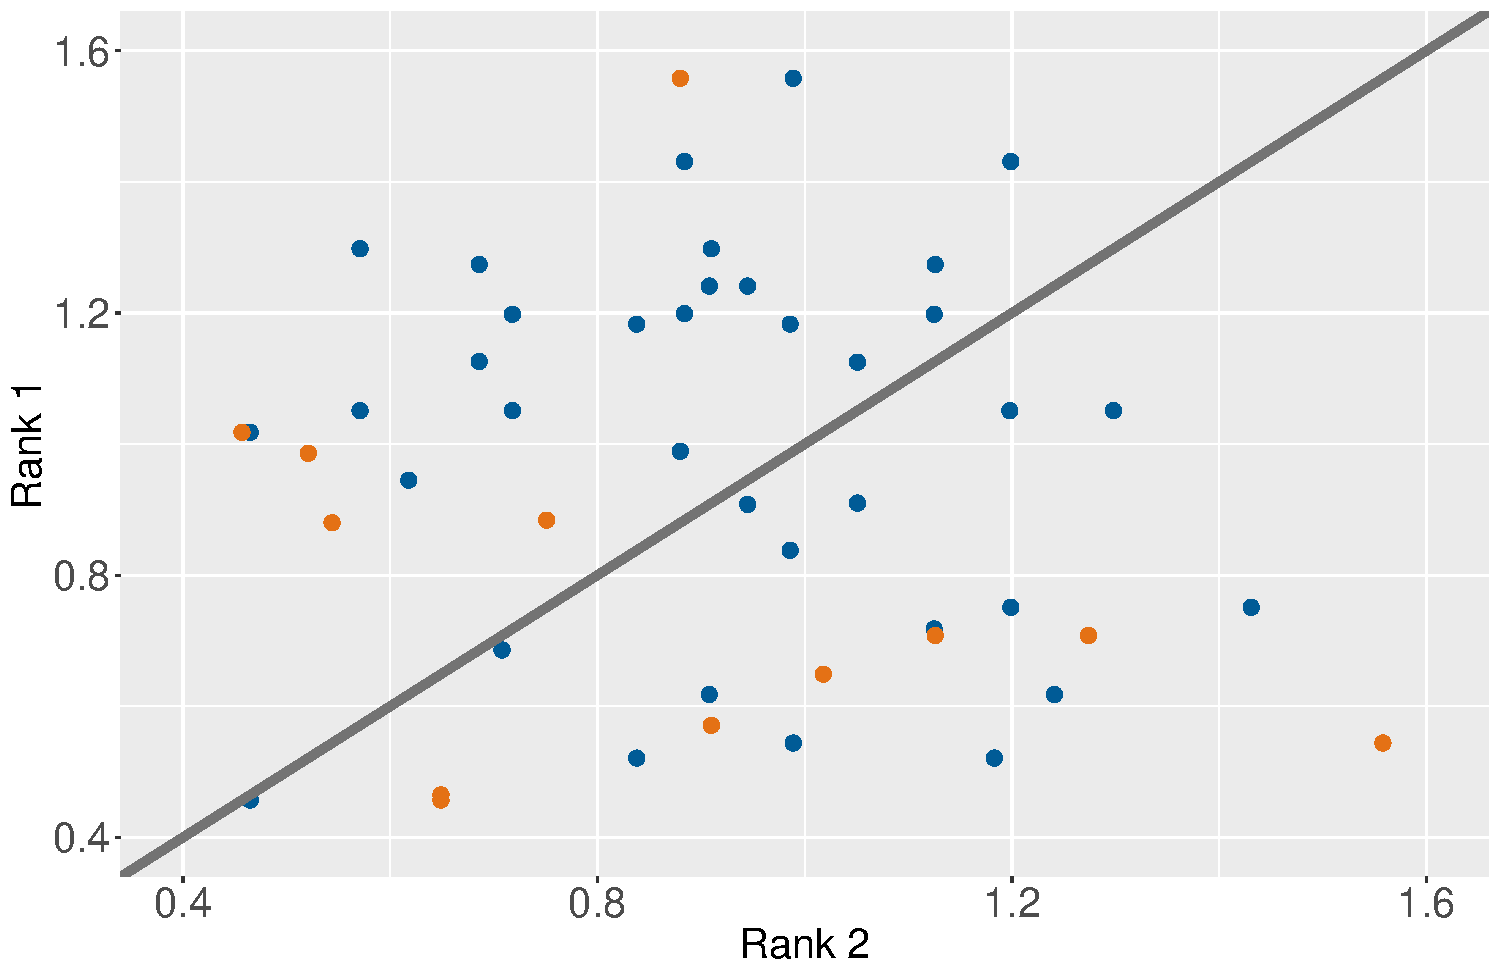
\includegraphics[scale=0.27]{ScenarioA.pdf}}~
\subfloat[Scenario B]
{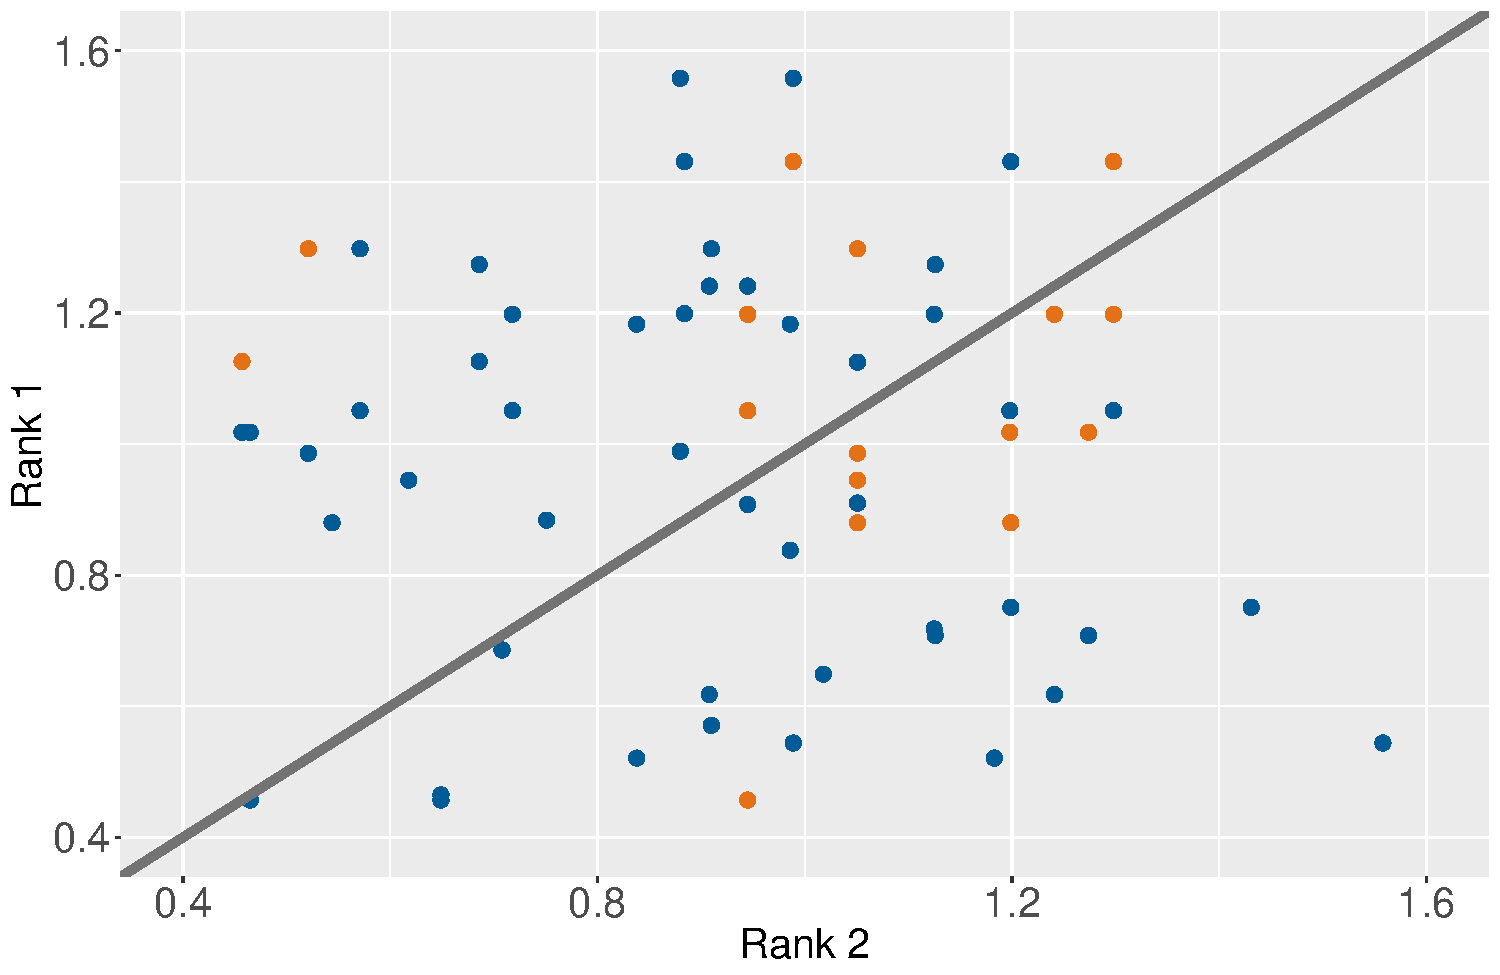
\includegraphics[scale=0.27]{ScenarioB.pdf}}\\
\centering
\subfloat[Scenario C]
{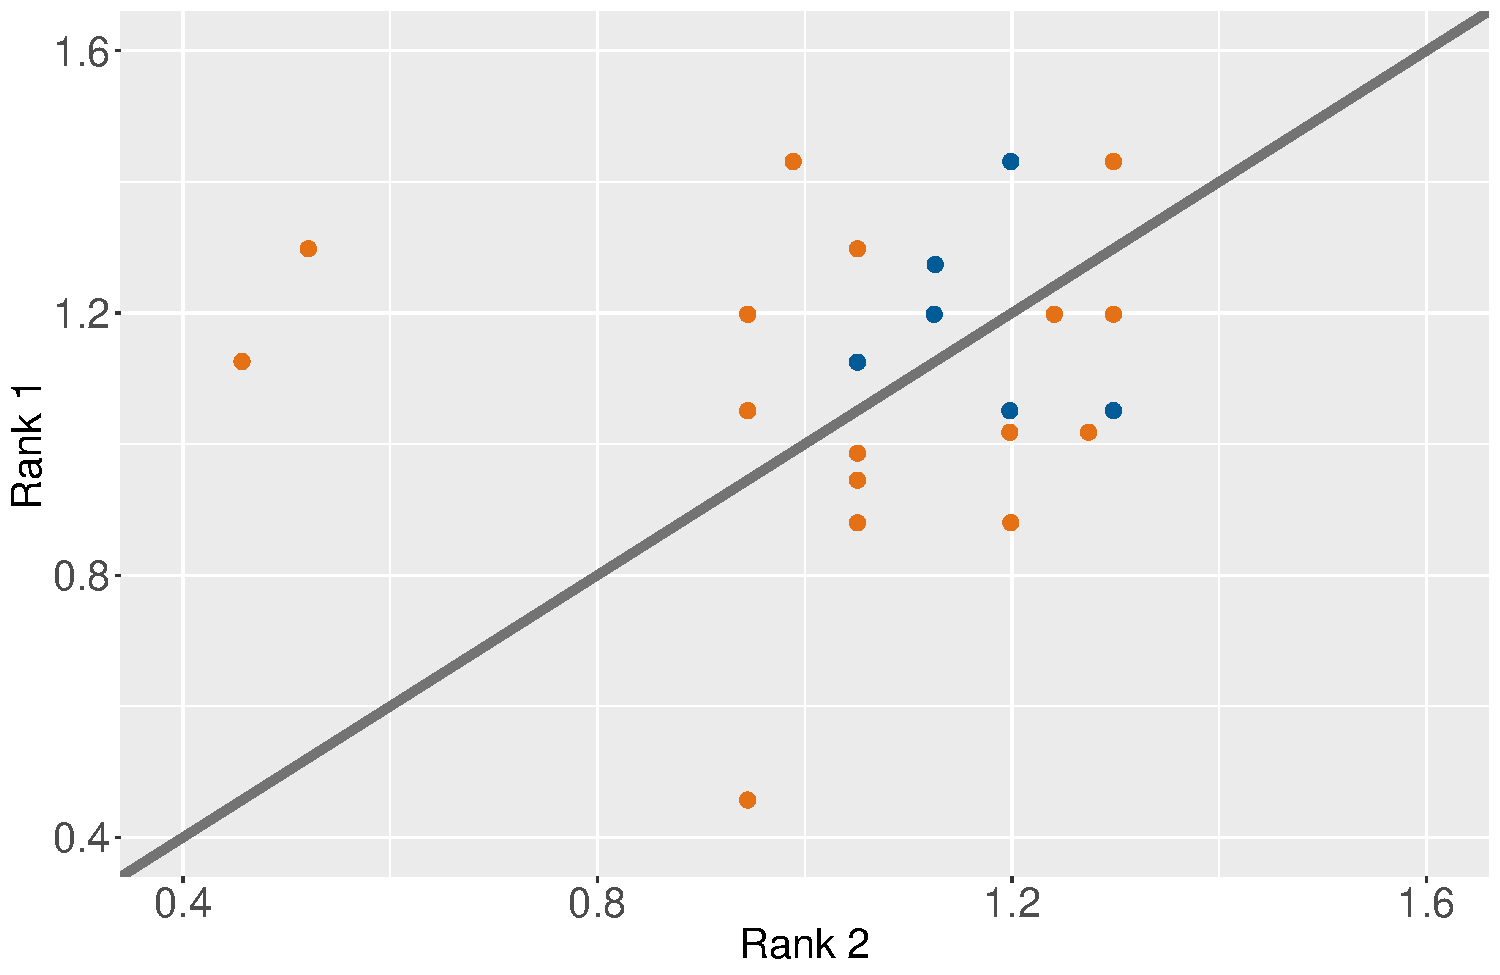
\includegraphics[scale=0.27]{ScenarioC.pdf}}
\caption{For each prediction scenarios, the values of the FIFA rankings for each match are shown in blue  for the training set and in orange  for the test set.}
\label{Fig1}
\end{figure}
\end{center}
%
\begin{figure}
\centering
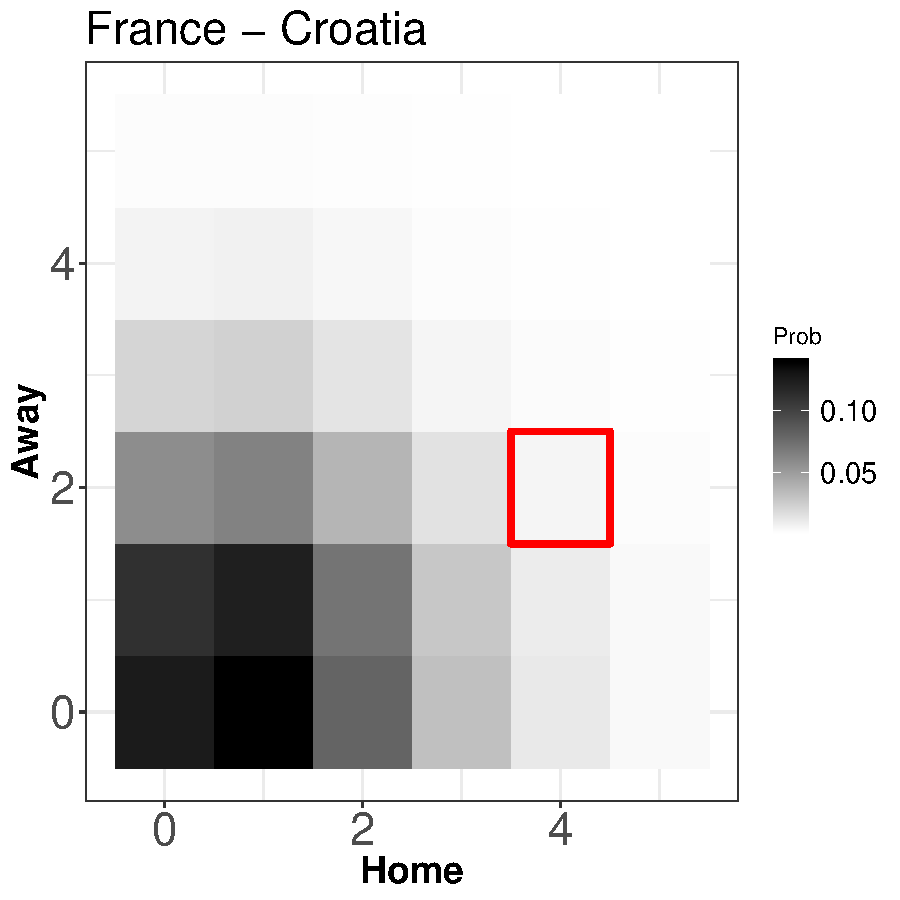
\includegraphics[scale=0.5]{France-CroatiaHeatmap_bivpois}
\caption{Posterior prediction distribution of the goals for the final France-Croatia}
\label{Fig2}
\end{figure}
%
Figure~\ref{Fig1} displays for each scenario the values for the FIFA rankings for the training set matches (blue points) and the test set matches (orange points), along with the 
line $\text{Rank }1= \text{Rank }2$, implying that the ranking difference is $w=0$. In Scenario A, the test set matches are randomly selected from the group stage, and they do not 
show any particular pattern around  line $w=0$. In Scenarios B and C, test set matches belong to the knockout stage, where the teams are expected to be stronger and 
closer to each other in terms of their rankings. In fact, the majority of the orange points (13 out of 16) is displayed towards the bottom right corner---higher rankings---and closer to the line $w=0$---closer strengths. Scenario B uses more and more data to predict test set results---all  48 group stage matches---whereas Scenario C only six matches.

Figure~\ref{Fig2} depicts the posterior predictive distribution (p5 and p7) of the number of goals scored by France and Croatia during the final from the bivariate Poisson model. Darker 
regions are associated with higher probabilities, whereas the red square  corresponds with the observed result, 4-2. From this plot, one could be tempted to 
conclude that the bivariate Poisson model completely failed to predict the match; however, the global probability of France winning within the 90 minutes---obtained summing the single probabilities over the lower triangle of the plot---is about 42\%, against the 29\% chance of winning for Croatia (p1 and p2). Fro this plot only we can acknowledge the intrinsic variability in our model predictions (p5).

To have a glimpse into statistical and ML procedures' predictive performance, Table 2 shows the accuracy in the predictions for the seven methods and the three  scenarios. Assuming that 
higher predictive accuracies should not entirely suggest the best scientific methods (p1), we analyse the performance of the methods by focusing on pro and cons. As suggested by 
Figure~\ref{Fig1}a, Scenario A is the  noisiest in terms of rankings' differences,  with the test set constituted by matches randomly chosen from the group stage, without any kind 
of pattern. As  is intuitive, ML techniques (Random Forest and Neural Nets), perform better, since they ``shake'' the training set (p8) in such a way as to retrieve the highest 
predictive accuracy. The ML performances dramatically decrease in Scenario B and C, where learning from the training set should be focused on predicting the knockout stage. ML algorithms learn less and in a very random way, but it is not clear why (p10).
As already argued, the choice of the training and the test set can dramatically 
change the predictive performance of the ML algorithms, which over-perform statistical models only when considering a portion of the group stage to predict the remaining 
group stage matches. Should  we perhaps conclude that statistical models are better scientific tools to predict the World Cup? Not at all (p1), but we can learn from this example to improve over the next World Cups (p4).

%Although the example is quite simple and the dataset is too small to extract general conclusions, there are enough arguments to emphasize the paradoxical performance achieved by ML techniques. Their predictive accuracy is too much influenced by the training set 
%structure, making impossible to draw conclusions about their plausibility for predicting the football World Cup. 
By concluding, from this simple case study we cannot openly 
falsify our statistical/ML techniques on the ground of future predictions. However, Poisson models seem to be less sensitive to the training set structure, and then falsifiable in a broader sense.

\begin{center}
\begin{table}
%\centering
\caption{Prediction accuracy for the selected methods, according to three prediction  scenarios.}
\begin{tabular}{|r|rrr|}
\hline 
 \emph{Train}& 75\% group  & 100\% group  & rank $>$ 1   \\ 
  \hline
\emph{Test} & 25\% group & knockout & knockout\\ 
  \hline
\emph{Random forest} & 0.67 & 0.25 & 0.44 \\ 
  \emph{Bagged CART} & 0.67 & 0.31 & 0.37  \\ 
%  bayesglm & 0.25 & 0.19 & 0.19 \\ 
  \emph{CART} & 0.58 & 0.31 & 0.19  \\ 
  \emph{MARS} & 0.58 & 0.38 & 0.49 \\ 
  \emph{NN} & 0.67 & 0.25 & 0.44  \\ 
  %Multinomial & 0.50 & 0.50 & 0.50 \\ 
  %Multinomial  & 0.42 & 0.62 & 0.62  \\ 
  \emph{Double Pois.} & 0.58 & 0.50 & 0.56  \\ 
  \emph{Biv. Pois.} & 0.58 & 0.56 & 0.56  \\ 
   \hline
\end{tabular}
%\label{tab1}
\end{table}
\end{center}
%

%Obviously it should be noted that the results presented here are only preliminary also considering the small size of the dataset here analysed. A full appreciation of the 
%different performances  is out-of the scope of the current paper and should be definitely considered for future research, also aimed  at defining a strategy for stacking models in this specific application case.

\section{Discussion}
\label{sec:concl}

Prediction is central in the progress of science and has become even more relevant in statistics and data science, as the availability of new 
computational tools has become common to accommodate data and predict new events. The entire field of science changed drastically over the last 
decades, new disciplines entered the scientific environment, and social sciences became a new frontier where predictive accuracy was required. 

Natural and physical sciences progressed with Popper's falsificationism  a main consequence of which is the 
strong predictivism: scientific theories should be falsified in light of wrong predictions. However, social sciences are not falsifiable in the 
same way: some social events---presidential elections, football results, and policy effects---are not perfectly predictable for many reasons, such 
as data origins and unpredictable human behaviors. In this paper, we relax the assumptions behind strong instrumentalism and we provide a 
several points (see Table 1) to frame statistical and ML techniques within a weak instrumentalist philosophy, in which the main 
proposals regard algorithm transparency and variability in predictions.

As statisticians required to build good models to accomodate complex data, we must warn statisticians and data science users about the role of prediction. Predictive accuracy is not always constitutive of scientific success: Prediction is not everything, but is vital, and it is our responsibility to choose the gun or the bazooka.



\bibliographystyle{chicago}
\bibliography{predbib}

\end{document}